% Familyties User Guide
%
% For PDF output: pdflatex familyties.tex
% For HTML output: plastex familyties.tex
%
% For Graphics:
% Use PNG format to avoid problems with HTML conversion.
% Recommended size: < 13cm x 18cm (width x height).
% Recommended resolution: 300 dpi.
%
% Use fixed width instead of textwidth, so that plastex can
% recognize the graphics size. For example use
% \includegraphics[width=13cm]{img/haplogroups.png}
% instead of
% \includegraphics[width=\textwidth]{img/haplogroups.png}

\documentclass[12pt,a4paper]{article}
\usepackage[utf8]{inputenc}
\usepackage[english]{babel}
\usepackage[colorlinks=true, urlcolor=blue, linkcolor=blue]{hyperref}
\usepackage{graphicx}

\begin{document}
\title{Familyties User Guide}
\author{Dirk Struve\\
phylofriend at projectory.de\\
\href{https://github.com/yogischogi/familyties/}{https://github.com/yogischogi/familyties/}}
\date{\today}
\maketitle
\tableofcontents

\section{Introduction}
Familyties is a program to analyse Family Tree's Family Finder
matches files. You can use it to
\begin{enumerate}
\item determine how many of your cousins have ancestry from which
  country.
\item find out how your family is connected to other parts of the
  world.
\item perform detailed analysis on parts of your family specified
  by surname or location.
\item discover ethnic origins of your family and yourself.
\item see which surnames are most frequent in your family.
\end{enumerate}


\section{Command Line Options}

Familyties is a command line program. It is invoked by

\vspace{1em}
\noindent\texttt{familyties [options] <Family Finder matches file>}

\vspace{1em}
\noindent Options may be given in arbitrary order.

\begin{description}
\item[-help] Prints available program options.
\item[-details] Performs detailed analysis for locations
  and surnames.
\item[-min <min>] Prints only locations and names that occur at
  least \texttt{<min>} times.
\item[-cluster] Performs cluster analysis on the cousins
  who's ancestral surnames or locations match \texttt{<cluster>}.
\item[-exclude <exclude>] Excludes cousins who's ancestral surnames or
  locations match \texttt{<exclude>}.
\item[-csvout <filename>] Writes a table of locations in CSV format
  to a file. Useful to create a heat map.
\end{description}


\section{Installation}

\subsection{Windows}
For Windows there is a precompiled binary available but it
may not always be the latest version.
\begin{enumerate}
\item \href{http://www.projectory.de/genetics/familyties.zip}
  {Download the program} and unzip it into the same folder
  as your Family Finder results.
\item Open a command line interpreter and go to the previous
  directory. You can involve the familyties program directly.
  It is a simple command and does not change your Windows
  installation.
\end{enumerate}

\subsection{Linux Mint}
\begin{enumerate}
\item Make sure that the Go programming language is installed.
	You can install it by typing\\
	\texttt{sudo apt-get install golang}
\item Read the Go
	\href{http://golang.org/doc/install}{Getting Started}
	guide. Make sure to set your \emph{GOPATH} variable and
	include it in your \emph{PATH} so that Go programs can be
	found.
\item Fetch the familyties program with\\
	\texttt{go get github.com/yogischogi/familyties}
\item Install the program with\\
	 \texttt{go install github.com/yogischogi/familyties}
\end{enumerate}

\subsection{FreeBSD, Mac OS X}
\begin{enumerate}
\item Read the Go
	\href{http://golang.org/doc/install}{Getting Started}
	guide and install the Go programming language. 
    Make sure to set your \emph{GOPATH} variable and
	include it in your \emph{PATH} so that Go programs can be
	found.
\item Fetch the familyties program with\\
	\texttt{go get github.com/yogischogi/familyties}
\item Install the program with\\
	 \texttt{go install github.com/yogischogi/familyties}
\end{enumerate}


\section{First Usage}

\begin{enumerate}
\item Download your Family Finder matches file from Family Tree DNA
   in CSV (Comma Separated Values) format. You will find it at
   \emph{Family Finder - Matches - Download Matches, CSV
   (bottom right of the page)}
\item Open a command line interpreter and switch to the
   directory where your matches file resides.
\item Issue a command, for example\\
  \texttt{familyties N123456\_Family\_Finder\_Matches\_20140920.csv}\\
  You do not need to type in the full filename. Just start typing and
  hit the TAB key for auto completion.
\end{enumerate}


\section{How to Create a Heat Map}

\begin{figure}[ht]
\centering
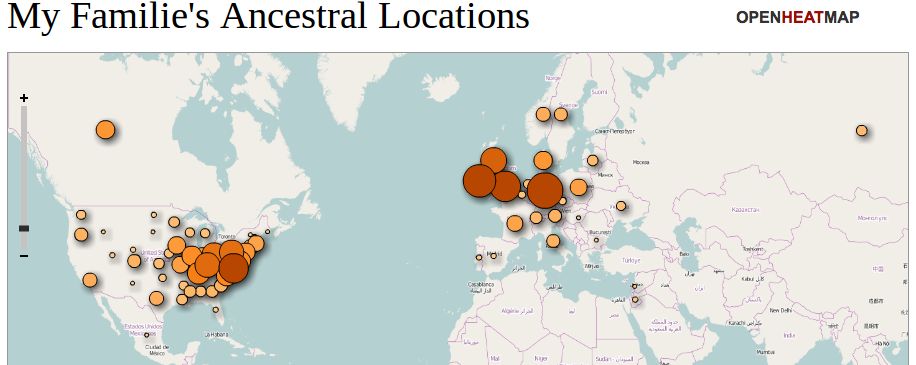
\includegraphics[width=13cm]{ancestral-locations.png}
\caption{Ancestral locations of my family. It is hard
to believe that this all happened within the relatively 
short time period of a genealogical time frame (about 400 years).}
\end{figure}

It is easy to create a heat map of your familie's ancestral locations
by saving the results to a file and upload them to
\href{http://www.openheatmap.com/}{OpenHeatMap}.
Here is how it is done:

\begin{enumerate}
\item Save the results to a file as Comma Separated Values:\\
  \texttt{familyties -csvout="Locations.csv"  N12345\_Family\_Finder\_Matches.csv}
\item Open your web browser and go to
      \href{http://www.openheatmap.com/}{http://www.openheatmap.com}.
	\begin{enumerate}
	\item Click on \emph{Create your map}.
	\item \emph{Excel or CSV file}.
	\item \emph{Upload} your results file,
            in this example \emph{Locations.csv}.
	\item \emph{View your map} and adjust the settings until you like it.
	\item \emph{Save \& view}
	\end{enumerate}
\item You are done! You can share your map via social networks
  or take a screenshot of it.
\end{enumerate}


\section{Examples}

\begin{enumerate}
\item Show how many of your cousins have ancestry from which
   country:\\
   \texttt{familyties N123456\_Family\_Finder\_Matches\_20140920.csv}
\item Save the results into the file \emph{family.txt}:\\
   \texttt{familyties N123456\_Family\_Finder\_Matches\_20140920.csv\\ > family.txt}
\item Show also the names of your cousins' ancestors:\\
   \texttt{familyties -details\\ N123456\_Family\_Finder\_Matches\_20140920.csv}
\item Show only ancestral names that occur at least five times:\\
   \texttt{familyties -details -min=5\\ N123456\_Family\_Finder\_Matches\_20140920.csv}
\item Show how many of your cousins have ancestry from which
   country, but exclude all who have ancestry from the USA:\\
   \texttt{familyties -exclude usa N123456\_Family\_Finder\_Matches\_20140920.csv}\\
   Because of the large migrations from Europe to the USA the results
   are often significantly distorted if you want to find out something
   about your European ancestry only. In this case the exclude option
   is very useful.
\end{enumerate}


\section{Example Session}

I want to get a first overview and start by typing:

\vspace{1em}
\noindent\texttt{familyties N123456\_Family\_Finder\_Matches\_20140920.csv}

\vspace{1em}
\noindent This yields:

\begin{verbatim}
--- Quick search for predefined countries ---
Number of cousins:  Ancestry from:
59 USA
42 Germany
28 England
28 Ireland
21 Scotland
10 France
8 Denmark
8 Poland
7 Norway
\end{verbatim}

From the results you might guess that I am either from the
USA or Germany (I am German). 59 of my cousins have ancestry
from the USA. I bet most of them are still there. I take a
closer look by examining the USA cluster in detail and write
the result into a file called \emph{results.txt}:

\vspace{1em}
\noindent\texttt{familyties -details -cluster=USA \\
N123456\_Family\_Finder\_Matches\_20140920.csv > results.txt}

\begin{verbatim}
--- Detailed analysis of ancestral locations ---
Number of cousins:  Ancestry from:
51 usa
22 germany
19 virginia
18 north carolina
\end{verbatim}

Now I know that many of them have ancestors from Virginia
and North Carolina. I examine the Virginia cluster in detail
because I am interested in the surnames:

\vspace{1em}
\noindent\texttt{familyties -details -cluster=Virginia \\
N123456\_Family\_Finder\_Matches\_20140920.csv > results.txt}

\begin{verbatim}
--- Detailed analysis of ancestral surnames ---
Number of cousins:  Ancestral surname:
7 white
6 smith
6 jones
\end{verbatim}

As expected the very common names come first (I left out
the rest). Usually you would look for a high occurrence
of less common names. This can yield some very detailed
information sometimes. 

Of course there is still much more information hidden in 
my results but I think this is enough to get you started.


\section{How You Can Help}

\begin{enumerate}
\item Provide ancestral information about yourself. Even if
  you do not have much information about your ancestors or
  think it is not important. Your cousins might be grateful
  for every piece of information. All these tiny pieces
  together show the whole family story.

\item Provide country names in English. A country usually has
  different names in different languages. Do not expect your
  cousins to speak the same language as yourself. So it is a
  good idea to provide an English name. You can also provide
  the native spelling and separate both names by commas.

\item Do not use fancy characters like slashes and braces.
  Use commas to separate different spellings of a name or
  towns and countries. Slashes and braces are used in the
  Family Finder matches file to separate entries. If you 
  use such characters for your own purposes the format gets
  invalid and the familyties program can not parse the
  information correctly. Surnames and locations get mingled.
  You will see this sometimes when looking at the
  program's results.

\item Do not use abbreviations. Although the familyties
  program recognizes US state abbreviations your cousins
  might not. Generally it is a bad idea to use abbreviations.
  They often have different meanings in different countries.
\end{enumerate}



\end{document}
